\section{Taxonomy similarity}

In this section, we propose a function to quantify the similarity between two strings based on a taxonomy tree and then propose several efficient string join algorithms. Here we assume that each string match a single node in the taxonomy tree and we extend it to multiple nodes in the next section.


\subsection{Similarity functions}

We borrow the labeling scheme from XML databases and use the prefix based labels. Dewey code is prefix-based labeling scheme that records the position information of each node, according to the path from the root to the node. Structural relationships between tree nodes whose positions are recorded in this fashion can be determined easily for IS-A relationships.



\begin{definition}[Taxonomy Similarity]
Given two nodes $n_1$ and $n_2$ on a taxonomy tree $\mathcal{T}$, the taxonomy similarity between $n_1$ and $n_2$, called NS($n_1$,$n_2$), is defined the longest common prefix (LCP) of  $n_1$ and $n_2$ over the length of the longer path between $n_1$ and $n_2$, that is,  NS($n_1$,$n_2$,$T$) = $\frac{|LCP(n_1,n_2)|}{max(|n_1|,|n_2|)}$. \end{definition}

\smallskip
\smallskip


\begin{example}
Consider Figure \ref{fig:taxonomyexample}, the similarity between ``\textsf{Seoul}'' (3.1.1.1) and ``\textsf{Suwon}'' (3.1.1.2) is $\frac{3}{4}$= 0.75 (as both countries are in South Korea.), and the the similarity between ``\textsf{Seoul}''  (3.1.1.1) and ``\textsf{Shenzhen}'' (3.2.1.1) is only $\frac{1}{4}$= 0.25 (as two countries are in Asia).
\end{example}

The complexity to computer TS is $O(|n_1|+|n_2|)$. This is efficient.



\subsection{Join algorithms for sorted lists}

We would formulate the string similarity join problem and develop the corresponding algorithms. Given two collections of strings $S$ and $T$, a taxonomy tree
$\mathcal{T}$, and a similarity threshold $\theta$, a \textit{string
  similarity join} finds all string pairs $(s, t) \in S \times T$,
such that $TS(s,t,\mathcal{T})$ $>$ $\theta$, where \textit{TS} is
 the taxonomy similarity functions defined above.



Given two collections of strings $S$ and $T$, the baseline join algorithm is the nested-loop join. All string pairs are accessed to determine the IS-A relationships. But this algorithm is obviously not efficient. Therefore, we propose an efficient algorithm.

The complexity to computer the join set is $O(|S| \cdot |T| \cdot L^2)$, where L is the longest string in the set. This is not efficient.



The first join method is based on the sort of data.

Associated with a collection $T$ there is a list $L_T$. This list contain the positional representation of the taxonomy tree nodes that match strings in the $T$. The nodes in the list are sorted by the lexicographical order. The operation over lists are: Eof, advance, next.
We main two cursors in each list: C1 and C2.

\begin{lem} Given a string $s$ with the length $|s|$, if any string t, $TS(s,t) > \theta$,  then $s$ and $t$ share the prefix with the length of at least $|s| \cdot \theta $.
\end{lem}

To speedup the query processing, we add two operators: $Len(e)$ is the length of the label $e$, and $LCPL(e)$ is the length of LCP($e,e'$), where $e'$ is the previous label of $e$. 

\begin{theorem} The TS join based on sorted lists perform the join for two table $S$ and $T$ in $\mathcal{O}$$(\Sigma LCP(R)+|S||T|)$. 
\end{theorem}
\begin{proof}  
\end{proof}

\subsection{Join algorithms with compact tries}

The second join method is based on compact tries.

Trie is a rooted tree with the following properties: Edges are labelled with symbols from an alphabet $\Sigma$
For every node $v$, the edges from $v$ to its children have different labels. Each node represents the string obtained by concatenating the symbols on the path from the root to that node. The space requirement can be problematic, since typically each node needs
much more space than a single symbol.



Compact tries reduce the number of nodes by replacing branchless path segments with a single edge.

%\begin{figure}[t]
%\centering
%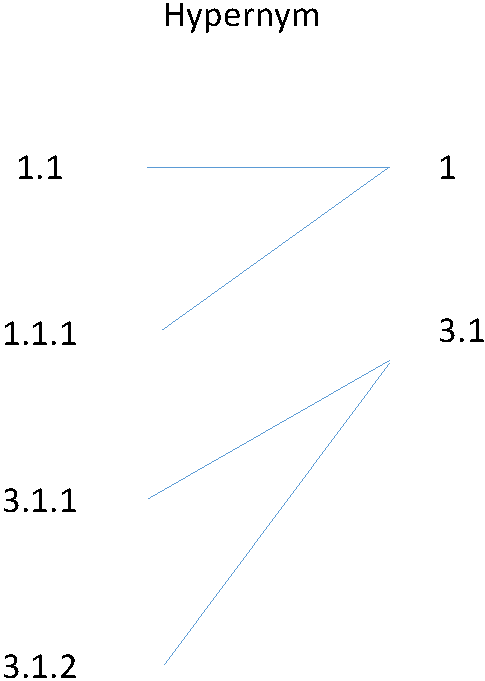
\includegraphics[scale=0.4]{figures/labeljoins}
% \caption{Join inverted lists}
%\label{fig:invertedlist}
%\end{figure}



\begin{algorithm}
{\bf Input}: two sorted lists of labels $L_1$ and $L_2$\\
{\bf Output}: pairs $(s_1,s_2) \in L_1 \times L_2$, s.t. $TS(s_1, s_2) > \theta$
\begin{compactenum}[(1)]
\item {\bf FOR}  i =1 and 2 {\bf DO}
\item ~~ Initialize two pointers $C_i^1$ and $C_i^2$ to the first element of  $L_i$
\item {\bf WHILE}  $\neg$end($L_1$) and $\neg$end($L_2$) {\bf DO}
\item ~~ $min$ = $\arg\min_{i}$($cur(L_i,C_i^1)$); $max$ = $\arg\max_{i}$($cur(L_i,C_i^1)$)
\item ~~ $p$ = prefix(cur($L_{min}$,$C_1^{min}$),$  \lceil l \cdot \theta \rceil$)
\item ~~ {\bf WHILE} (cur($L_{max}$,$C_2^{max}$) has the prefix $p$) {\bf DO}
\item ~~ ~~ ~~ {\bf IF} TS(cur($L_{max}$,$C_2^{max}$), cur($L_{min}$,$C_1^{min}$))$> \theta$ {\bf THEN}
\item ~~~   ~~ ~~ ~~ Add this pair to $R$
\item ~~ ~~ ~~  advance($L_{max}$,$C_2^{max}$)
\item ~~ $L_{max}.C_2$ =$L_{max}.C_1^{max}$
\item ~~ advance($L_{min}$,$C_1$)
\end{compactenum}
\smallskip
\textbf{Function} end($L_i$)
\begin{compactenum}[(1)]
\item {\bf IF}  cur($L_i$,$C_i^1$) is the last element of $L_i$ {\bf THEN}
\item  ~~ RETURN TRUE 
\item  {\bf ELSE} FALSE
\end{compactenum}
\caption{TS Join based on sorted labels}
\label{alg:exactjoin}
\end{algorithm}

The worst case complexity is $O(N^2)$, because the algorithm may compute each pair of strings with the prefix $p$. But this algorithm will skip many pairs of string for comparison. A theoretical analysis based on a random string model show that the average complexity is $O(\frac{N^2}{S^{\lfloor (1-\theta) \cdot l \rfloor}})$, where $N$ is the total number of elements in each list and $S$ is the maximal width of the taxonomy.



\begin{figure}[t]
\centering
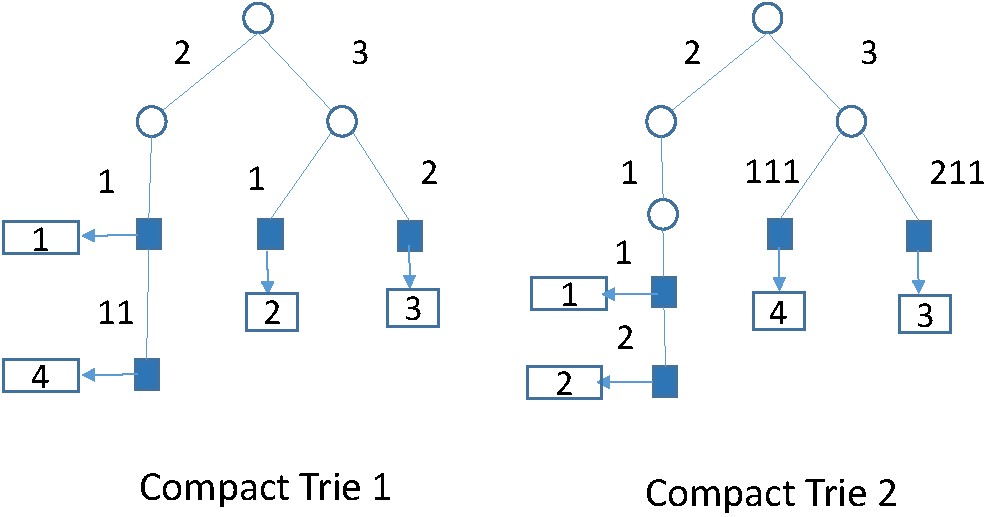
\includegraphics[width=0.35\textwidth]{figures/prefixTrees}
 \caption{An example of TS join based on prefix trees (a circle means an internal element, but a rectangle means a real element)}
\label{fig:taxonomyexample}
\end{figure}


\begin{algorithm}
{\bf Input}: two sets of strings $S$ and $T$, a taxonomy $\mathcal{T}$, a threshold $\theta$ \\
{\bf Output}: string pairs $(s_1,s_2) \in S_1 \times S_2$, s.t. $TS(s_1, s_2) > \theta$
\begin{compactenum}[(1)]
\item Let $T_s$ and $T_t$ denote two prefix trees for $S$ and $T$ respectively.
\item {\bf WHILE} $\neg end(T_s) \vee \neg end(T_t)$ {\bf DO}
\item ~~ Let $T_{min}$ denotes the list with the smaller elements and $T_{max}$ is the larger
\item  ~~ {\bf IF} (possibleMatch(cur($T_{min}$),cur($T_{max}$))) {\bf THEN}
\item ~~ ~~ {\bf  IF} ($T_{min}$ is a real element)   {\bf THEN} Find(cur($T_{min})$,cur($T_{max}$))
 \item ~~~~ advance($T_{min}$)
 \item ~~ {\bf ELSE} Jump($T_{min}$)
\end{compactenum}
\smallskip
\textbf{Function} possibleMatch($s_1$,$s_2$)
\begin{compactenum}[(1)]
\item  $x = LCP(s_1,s_2)$
\item {\bf IF}  $(x > \theta \cdot min (s_1, s_2 )$  {\bf THEN}
\item  ~~ RETURN TRUE
\item   {\bf ELSE} FALSE
\end{compactenum}
\smallskip
\textbf{Procedure} Jump($T$)
\begin{compactenum}[(1)]
\item  read the next element that is not a descendant with the depth-first traversal
\end{compactenum}
\smallskip
\textbf{Procedure} Find($s_1$,$s_2$)
\begin{compactenum}[(1)]
\item  $x = LCP(s_1,s_2) $
\item {\bf IF} ( $|s_2| < max(\frac{x}{\theta},|s|)$) {\bf THEN}
\item ~~~~ {\bf FOR EACH} $i$=$|s_2|$ to $ \lceil max(\frac{x}{\theta},|s|) \rceil -1 $ {\bf DO}
\item ~~~~~~~ Add all real nodes under $s_2$ with the length $i$ to R;
\end{compactenum}
\caption{String joins with taxonomy}
\label{alg:exactjoin}
\end{algorithm}


\begin{lem} Given two labels $s$ and $t$,  assume that $LCP(s,t) = x$. without the loss of generality, assume that $s<t$ by the lexicographical order, $TS(s,t) > \theta$ if and only if  $ x > \theta |s| $ and $  |t| < max(\frac{x}{\theta},|s|)$.
\end{lem}
\begin{proof}  $TS(s,t) > \theta$ $\Leftrightarrow$ $\frac{x}{|s|+|t|-x} > \theta \Leftrightarrow |t| < (\frac{1}{\theta}+1)x-|s|$. In addition, note that $|t| \geq x$. Then $x < (\frac{1}{\theta}+1)x-|s|$ $\Rightarrow$ $x > \theta |s| $, which concludes the proof.
\end{proof}


\smallskip
\smallskip

\begin{example}
Consider the example in Figure \ref{fig:taxonomyexample}, $\theta$=0.4. First, the cursors point to 2 and 2. possibleMatch return true. But 2 is not the real elements.  Then advance. Now $s_1$ =2.1 in $T_1$  and $s_2$=2.1.1 in $T_2$. Both real nodes. $x$=2.1, ($\frac{1}{\theta}+1)|x|-|s_1|$ = $5 > 3$. Therefore, (2.1, 2.1.1) and (2.1, 2.1.1.2) are added to the result pairs. Then the cursor advances, when $s_1$ =2.1.1.1, the result pair (2.1.1.1, 2.1.1.2) are added. Subsequently, the other two pairs (3.1, 3.1.1.1) and (3.2, 3.2.1.1) are added.
\end{example}

\smallskip
\smallskip


\begin{theorem}  Algorithm \ref{alg:exactjoin} is an optimal algorithm. The computing cost is linear to the sum of the size of the input and output. That is, each output result contribute to the final answer.
\end{theorem}




